\chapter[Benchmark orodja]{Benchmark orodja}

\pagestyle{fancy}
\fancyhf{}
\fancyhead[LE,RO]{\thepage}
\fancyhead[RE,LO]{\leftmark}

\huge Žiga Šebenik, Tomaž Mrežar
\normalsize
\bigskip

\section{Opis problema}
Za določanje zmogljivosti računalniških sistemov je na voljo veliko orodij, tako odprtokodnih, zastonjskih kot tudi plačljivih. V tem poglavju bova predstavila orodja in postopke, s katerimi sva midva testirala virtualni računalnik na Microsoftovem oblaku Azure, kjer sva imela odprt brezplačni račun. Na njem sva pognala različna bremena, kjer sva testirala omrežne povezave, diskovje in procesor. Nekaj od teh bremen sva ustvarila s pomojčje zastonjskih programov: Geekbench 3 za test procesorja, iPerf za test omrežja, ioPing za latenco diskovja in fio za test pasovne širine diskovja. Vsako orodje sva opisala in naštela prepoznavne značilnosti in prednosti pred ostalimi orodji. Ostala bremena sva ustvarila sama. Napisala sva namreč dva krata programa, enega za test omrežja in diska hkrati, ter enega za test moči procesorja. Ta dva programa sva pognala vsak na svojem računalnikiu, prav tako pa sva jih pognala tudi na virtualnem računalniku, da sva lahko primerjala zmogljivosti. Najina računalnika se razlikujeta v moči, saj je en računalnik prenosnik, drugi pa osebni računalnik, razlika pa je tudi v lokaciji, saj sva teste poganjala iz Kranja in Brezovice pri Ljubljani. Imava tudi različna ponudnika interneta, kar vse pride v poštev pri testih. Iz rezultatov testiranja sva nato poskušala sklepati o razlogih za razlike, ki so se pri teh testih pojavile.
  
\begin{figure}[H]
	\centering
	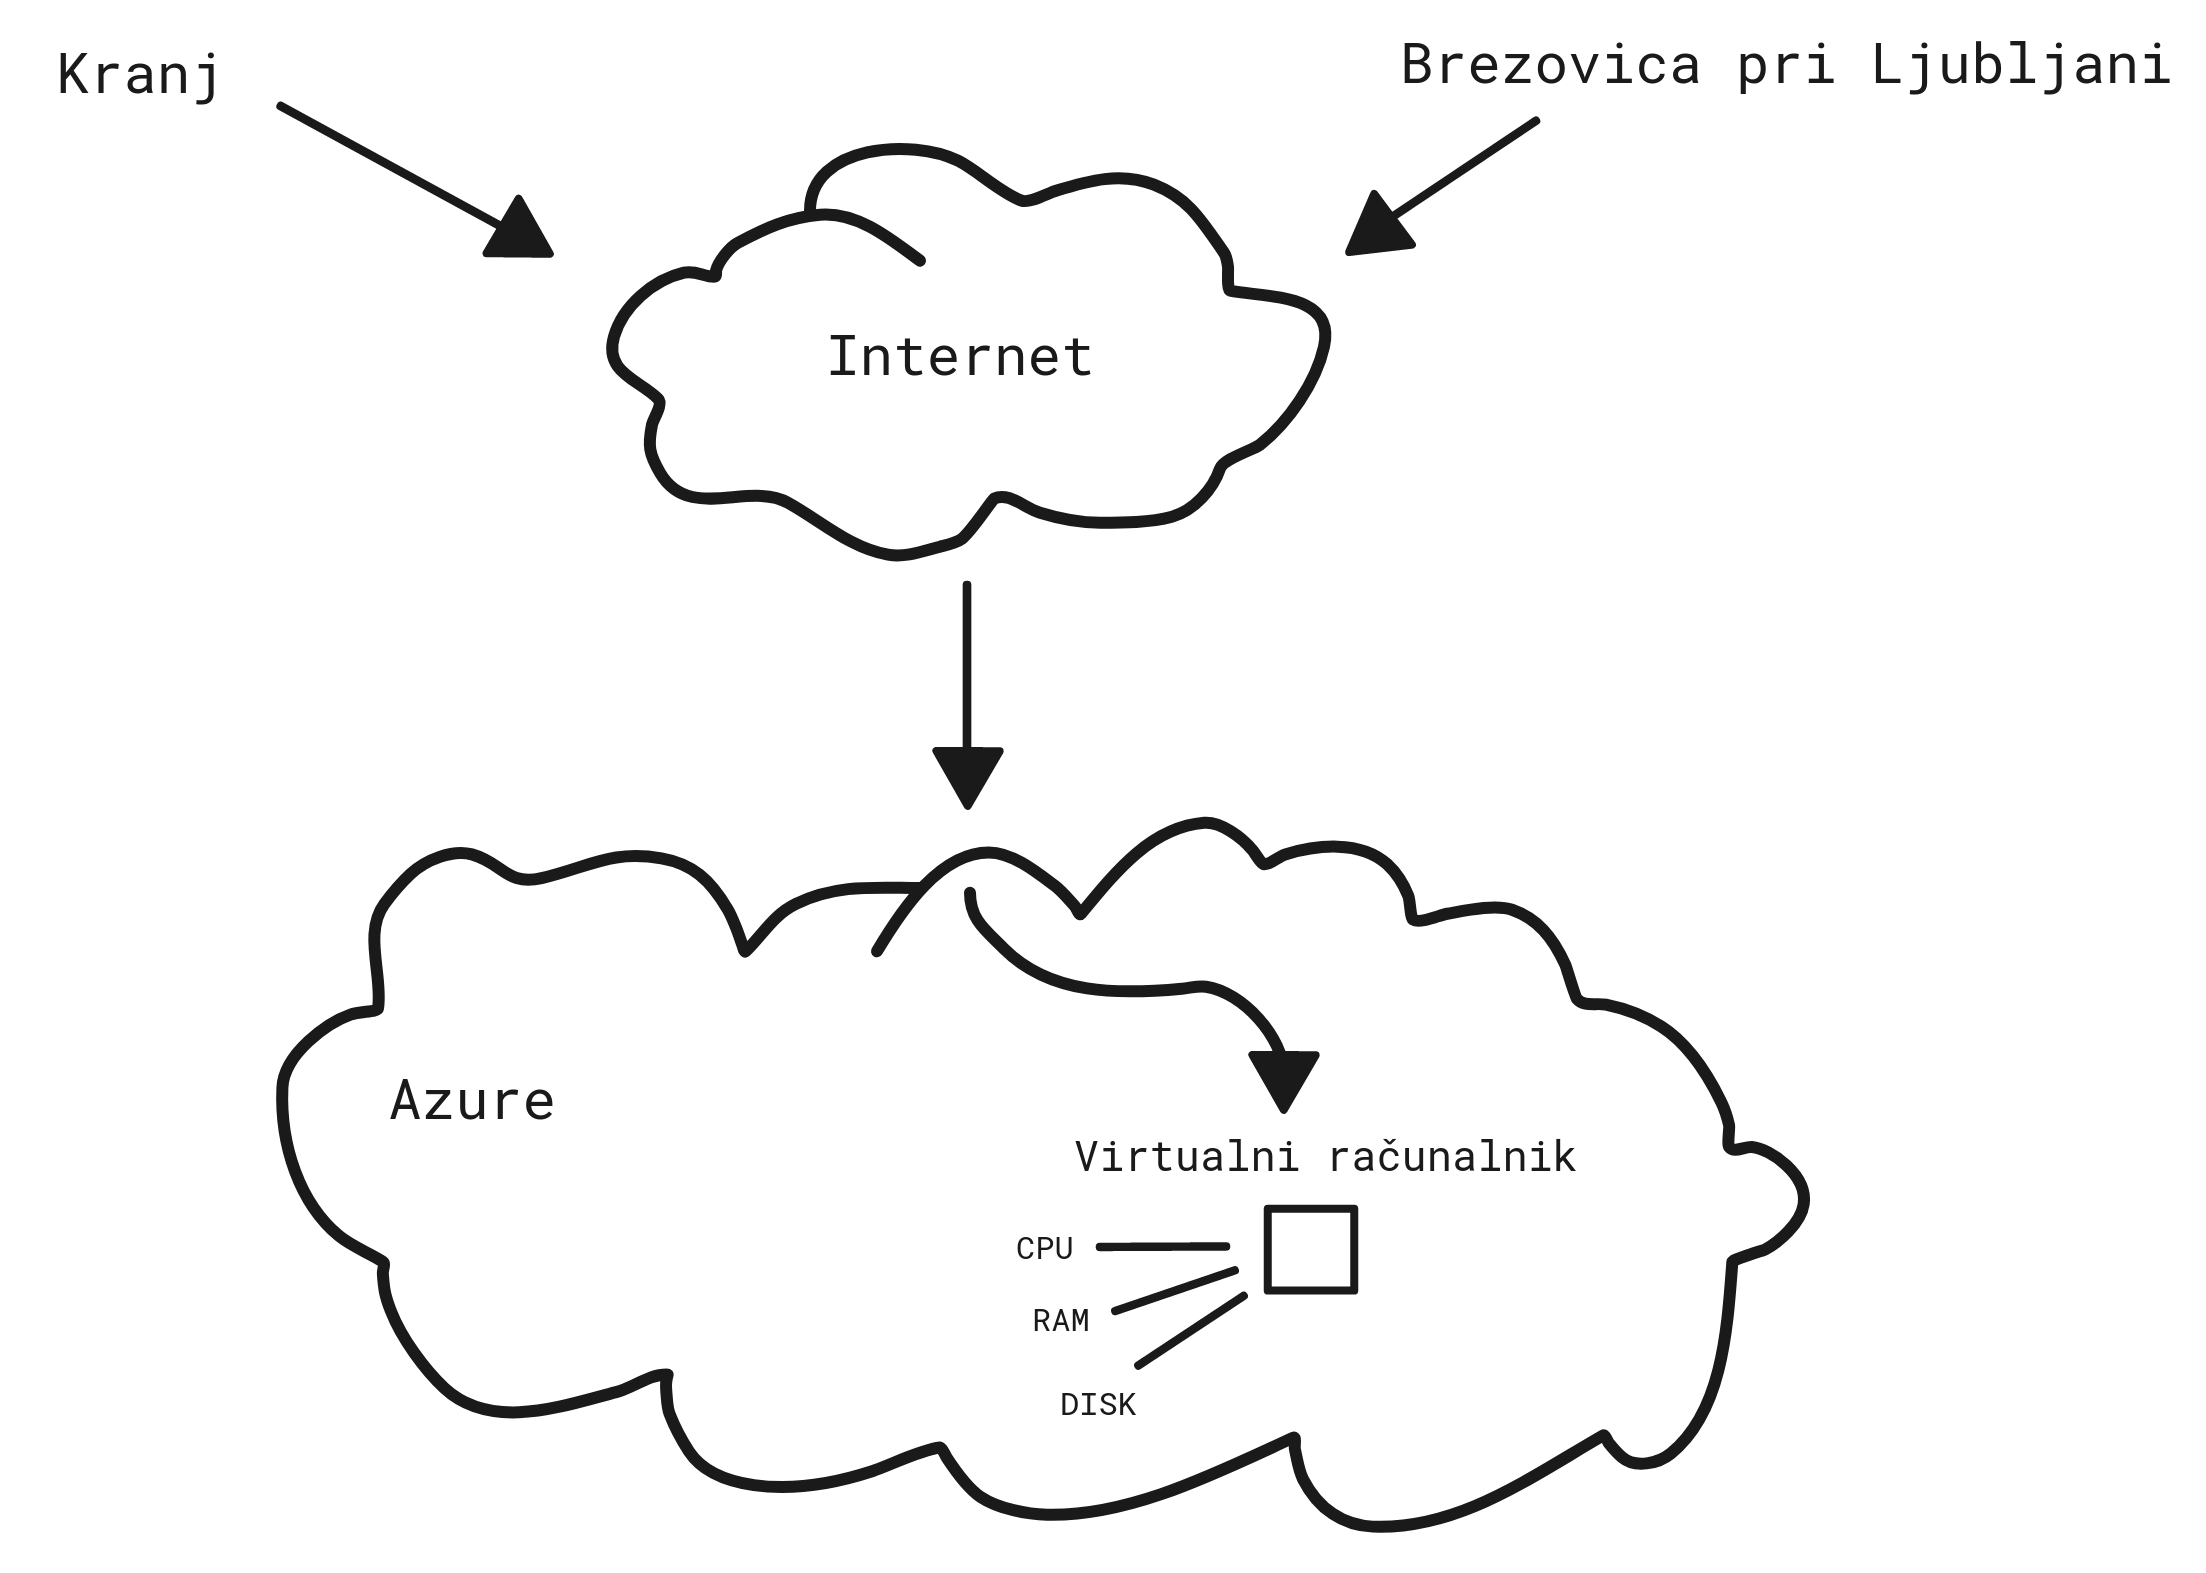
\includegraphics[scale=0.15]{Img/celotni_diagram.png}
	\caption{Celotni prikaz testiranja na Azure platformi.}
	\label{fig:7_breme2}
\end{figure}

\section{Benchmark orodja}
Obstaja več vrst benchmark orodij. Testi, ki jih benchmark orodja izvajajo se lahko razlikujejo med seboj vendar so osnovne funkcionalnosti testov skoraj povsod enake. Skorajda vsako orodje testira dosegljivost sistemov, upočasnitve delovanja, latenco sistema in prepustnost sistema. Orodja bova delila na dve skupini, prva skupina bodo orodja, ki so brezplačna, medtem ko bodo v drugo skupino spadala orodja, ki so plačljiva, brezplačna za določen čas ali pa imajo v brezplačni verziji omejene funkcionalnosti.

\section{Brezplačna orodja}
Brezplačni orodji sta sledeči:
\begin{itemize}
\item ročno benchmark testiranje;
\item PerfKit Benchmarker;
\end{itemize}

\subsection{Ročno benchmark testiranje}
Zelo preprosta izbira, ki nam je na voljo, je da preprosto sami testiramo zmogljivost oblačnih storitev s pomočjo več različnih orodij,pri čemer je vsako namenjeno specifičnemu delu sistema. Na voljo nam je veliko zastonjskih orodij, precej jih je tudi odprtokodnih, znani med njimi pa so ping, Geekbench, fio, iPerf... Testiramo lahko zmogljivost posameznega strežnika, gruče ali pa celotnega oblaka. Njihova prednost je, da so preprosta in fleksibilna, vendar pa moramo več dela opraviti sami.

\subsection{PerfKit Benchmarker}
PerfKit Benchmarker je odprtokodno orodje uporabljamo za meritve in primerjave oblačnih performans.
Podpira več večjih oblačnih ponudnikov, kot sta Google Cloud Platform in Amazon Web Services, pa tudi mnoge druge.
PerfKit Benchmarker meri končni čas za zagotavljanje virov v oblaku in tudi vse osnovne oblačne meritve naštete v predhodnem razdelku. PerfKit Benchmarker zmanjšuje kompleksnost v zaganjanju testov na oblačnih ponudnikih z enotnimi in preprostimi ukazi.
Vsebuje tudi množice javnih testov za uporabo. Vsi testi se zaženejo z privzeto konfiguracijo, ki ni nastavljena v prid nobenemu ponudniku oblačnih storitev. To ponuja možnost testiranja na več različnih oblačnih platformah.
V bistvu je Perfkit Benchmarker le orodje, ki avtomatizira zagon ostalih, ozko nameskih orodij za test posameznih metrik platforme. Vsa orodja, ki jih uporablja so odprtokodna in bi jih lahko pognali sami, vendar nam Perfkit Benchmarker, zmanjša količino dela, saj ima prilagojene skripte za vse večje ponudnike.

\section{Plačljiva orodja}
Plačljiva orodja so sledeča:
\begin{itemize}
\item SPEC Cloud® IaaS 2018;
\item Cloud Spectator;
\item Cloud Performance Benchmark;
\item Technology Business Research, Inc.;
\end{itemize}

\subsection{SPEC Cloud® IaaS 2018}

SPEC Cloud® IaaS 2018 testira delovanje infrastrukture kot storitev oblačnih implementacij. Podpira testiranje javnih in zasebnih oblakov. Orodje deluje nad strežbo storitve, kot tudi nad izvajanjem storitve oblaka z uporabo vhodno izhodnih in CPE intenzivnih del. Vsako delo se zažene kot distribuirana aplikacija narejena iz 6 ali 7 instanc, ki obremenijo oblakove resource (CPE, diski in omrežje). Delo bo teklo dokler testi ne naredijo več kakovosti storitve. Administrator lahko tudi omeji število aplikacij kreiranih med izvedbo.
Orodje nam omogoča obremeniti računsko zmogljivost, shrambo in omrežje oblaka. Pri tem pa ne potrebuje hypervizorja ali virtualizacijske plasti in uporablja delovne obremenitve, ki spominjajo na tiste, ki običajno delujejo v oblaku, kot so aplikacije za socialne medije in velika analiza podatkov.
SPEC Cloud izdaja poročila, ki ne grejo tako v detajle posameznega dela platforme ter izdajajo ločene metrike za vsak del platforme, ampak testirajo zmogljivost ponudikove platforme kot celote. Merijo čas stvaritve, konfiguracije in zagona instanc oz. virtualnih strojev, latenco vstavitve oz. branja iz baze na postavljeni virtualki, prepustnost, skalabilnost. Vse metrike so merjene v sekundah oz. operacijah na sekundo.

\subsection{Cloud Spectator}

Cloud Spectator sicer ni orodje, ampak podjetje, ki ponuja benchmarking in konzultacijo glede oblačnih storitev. Podjetjem pomaga z analizo različnih ponudnikov oblačnih storitev in testira zmogljivost njihove infrastrukture ter svetuje pri ekonomskih odločitvah. Namenjen je tako primerjavi ponudnikov oblačnih storitev, kot tudi ponudnikom samim, da lahko analizirajo zmogljivost svoje infrastrukture. Nudili naj bi sposobnost izbire pravega ponudnika, kjer stranka postavi zahteve svoje aplikacije, Cloud spectator pa s kombinacijo zahtevosti strankine aplikacije, zmogljivosti infrastrukture različnih ponudnikov in njihovih cenikov, izbere pravega ponudnika.
Poročilo vrača rezultate v obliki VM Performance Sore in CloudSpecs Score. Nobeden od njiju nima posebne merske enote, saj je VM Performance Score le povprečje točk, ki jih vrneta Geekbench 4 in fio, tako da imata oba enak prispevek k točkam. CloudSpecs Score se izračuna kot VM Performance Score, ki je utežen s ceno, tako da dobimo zmogljivost na ceno, ki naj bi strankam omogočala lažjo izbiro pravega ponudnika platforme.

\subsection{Cloud Performance Benchmark}

Cloud Performance Benchmark je poročilo o največjih petih ponudnikih Amazon Web Services, Google Cloud Platform, Microsoft Azure, IBM Cloud in Alibaba Cloud. Zagotavljalo naj bi nepristransko strokovno poročilo, ki je podprto z raznimi metrikami. Poročilo primerja infrastrukturo posameznega ponudnika in pokaže kako ta infrastruktura njihovega vpliva na zmogljivost ter jih seveda primerja med seboj. Prav tako se dotakne geografskih razlik in njihov vpliv na zmogljivost.
Poročilo ne vsebuje le kvantitativnih podatkov o posameznih platformah, temveč tudi veliko več kvantitativnih in statističnih podatkov o predvidljivosti posameznih metrik poleg razlag arhitektur vsake platforme. Poročilo je zelo poglobljeno, kvantitativne metrike pa se tičejo predvsem omrežja, saj je velik poudarek na latenci, tako izven kot znotraj platforme, ter izgubi paketov. Veliko podatkov najdemo tudi o vplivu geografskih pozicij na kakovost omrežja vsake platforme, vse podprto z statistično analizo obeh metrik.

\subsection{Technology Business Research, Inc.}

Technology Business Research, Inc. je podjetje, ki prav tako nudi storitve tako ponudnikom oblačnih storitev, kot tudi njihovim strankam. Ponudnikom nudijo podatke o trgu, finančne podatke o ponudnikih programske opreme, napovedi, strategije prodaje, itd. Ponudnikom oblačnih storitev pa nudijo podatke o ponudnikih le teh storitev, zmogljivosti ponudnikove infrastrukture za strankin primer uporabe ter tudi prihajajoče trende, ki se bodo posluževali in vplivali na zmogljivost oblačnih sistemov.
TBR Inc. je bolj usmerjeno v svetovanje situaciji na trgu, kot pa poglobljeni analizi metrik in zmogljivosti. Sledijo trendom in priložnostim na trgu, napovedujejo nove trende in sledijo finančnim podatkov ponudnikov platform. Njihov glavni cilj je direktni stik in osebno svetovanje strankam, zato nisem uspel najti nobenih uporabnih podatkov o njihovi metodologiji oz. metrikah.


\section{Implementacija merilnega okolja}
Na oblaku Microsoft Azure sva ustvarila račun in na njem postavila virtualni stroj, ki poganja Ubuntu 18.04. Na tej virtualki sva ročno pognala več benchmark testov, saj googlov odprtokodni Perfkit Benchmarker ni deloval. Le ta se namreč zanaša na avtomatsko ustvarjanje virtualnih strojev, zastonjski račun na Azure pa to omejuje. Pognala sva odprtokodna orodja:
\begin{itemize}
\item Geekbench 3 = uporabljen predvsem za test CPE zmogljivosti;
\item  test pasovne širine omrežja in dostop do interneta;
\item  latenca diskovja;
\item  zmogljivost diskovja;
\end{itemize}

\subsection{Tehnične specifikacije računalnika}
Specifikacije računalnika na katerem teče virtualni stroj so sledeče:

\begin{itemize}
\item OS: Ubuntu 18.04.4 LTS 5.0.0-1032-azure x86\_64
\item CPE: Intel Xeon Platinum 8168 @ 2.69 GHz 1 processor, 2 threads
\item RAM: 4 GB
\item Disk: 32 GB SSD
\end{itemize}
Ker se računalnik nahaja nekje v Microsoftovem strežniškem centru in ker uporabljava zastonjski račun na Azure, nimava na razpolago celotnega računalnika, saj na njem verjetno teče tudi kakšna druga virtualka, kar zna vplivati na rezultate meritev. Omenjene specifikacije računalnika so le te, ki jih imava na voljo na virtualki.


\section{Rezultati meritev}

V naslednjih razdelkih bova predstavila testna orodja uporabljena na virtualnem računalniku in dobljene rezultate.

\subsection{Geekbench 3}
Najprej sva pognala Geekbench 3, benchmark, ki se uporablja za testiranje CPE zmogljivosti. Imel naj bi to prednost pred klasičnimi testi CPE, da simulira tako breme na procesorju, ki dobro ponazarja produkcijsko okolje med izvajanjem realnih programov, in ne samo sintetični breme. Prav tako Geekbench dodobra obremeni računalnik, da lahko vidimo zmogljivost ob velikem stresu. Še ena dobra stvar kar se tiče Geekbench-a je, da je zelo razširjen, kar pomeni da lahko najdemo veliko različnih rezultatov testov za različne konfiguracije računalnikov, vendar pa to ne pomeni da je zanesljiv. Obstajajo namreč primeri, kjer ima strežniški CPE slabšo oceno kot nek mobilni CPE, saj Geekbench ne testira termalnih zmogljivosti, prav tako pa so razlike med rezultati na različnih operacijskih sistemih. Čeprav Geekbench uporabi več različnih testov, iz povzetka vseh teh testov vrne dve glavni številki: Single-core točke in Multi-core točke, ki sami po sebi nič ne pomenita in nimata merskih enot, velja pa višje je, bolje je. Šele ko ju primerjamo z ostalimi sistemi, dobimo neko sliko zmogljivosti. 

Na sliki \ref{fig:1_geekbench1} so predstavljeni rezultati večih algoritmov za performanse celih števil. Algoritmi se izvajajo na enem jedru procesorja in na večih.
\begin{figure}[H]
    \centering
    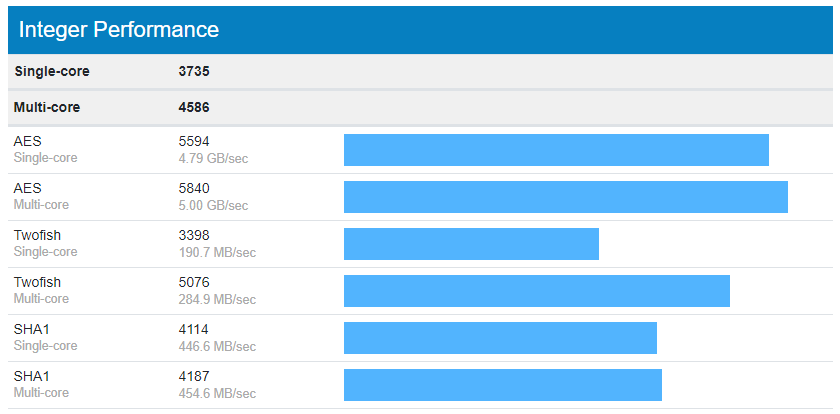
\includegraphics[scale=0.5]{Img/geekbench1.png}
    \caption{Cela števila.}
    \label{fig:1_geekbench1}
\end{figure} Na sliki \ref{fig:2_geekbench2} so predstavljeni rezultati večih algoritmov za performanse števil v plavajoči vejici. Algoritmi se izvajajo na enem jedru procesorja in na večih.
\begin{figure}[H]
    \centering
    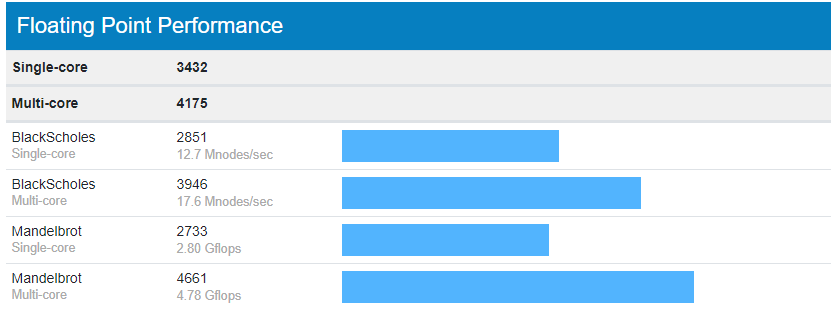
\includegraphics[scale=0.5]{Img/geekbench2.png}
    \caption{Plavajoča vejica.}
    \label{fig:2_geekbench2}
\end{figure} Na sliki \ref{fig:3_geekbench3} so predstavljeni rezultati za testiranje spomina. Testira se z kopiranjem na večih jedrih in na enem jedru procesorja.
\begin{figure}[H]
    \centering
    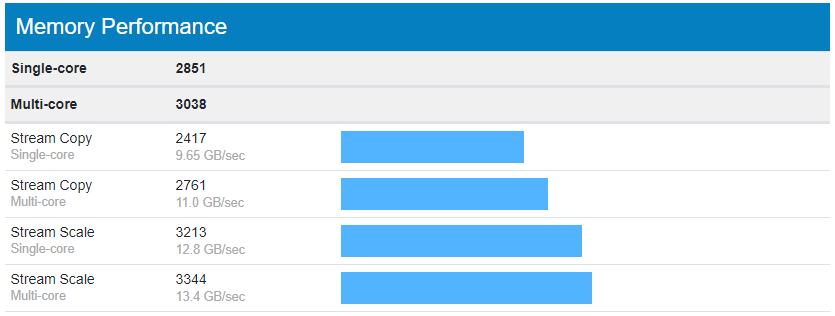
\includegraphics[scale=0.5]{Img/geekbench3.png}
    \caption{Performanse spomina.}
    \label{fig:3_geekbench3}
\end{figure}

\subsection{iPerf}
Naslednji benchmark, ki sva ga pognala je iperf, ki meri podatke o omrežju kot sta upload in download pasovno širino. Meri jih v bajt/sekunda, kjer prilagodi prefix od bajta glede na hitrost omrežja. Test sva pognala nad omrežjem med nama in virtualnim strojem. Čeprav bi lahko v najinem primeru podatke popačila hitrost ponudnika interneta na najini strani, pa temu verjetno ni tako, saj sva testirala na omrežju z 12 MB/s prenosa. Nisva prepričana, ali isto velja tudi za upload hitrost, latence pa nisva testirala, saj se strežnik nahaja na nizozemskem in latenca zaradi geografske lokacije pač je kakršna je. Iperf nama vrne povprečno hitrost prenosa podatkov 2,71 MB/s in 2,53 hitrost uploada podatkov, kjer velja, da večje številke pomenijo boljše performanse. Na sliki \ref{fig:4_iperf1} so predstavljeni rezultati testa iPerf, kjer lahko vidimo hitrosti prenosa na intervalih.
\begin{figure}[H]
    \centering
    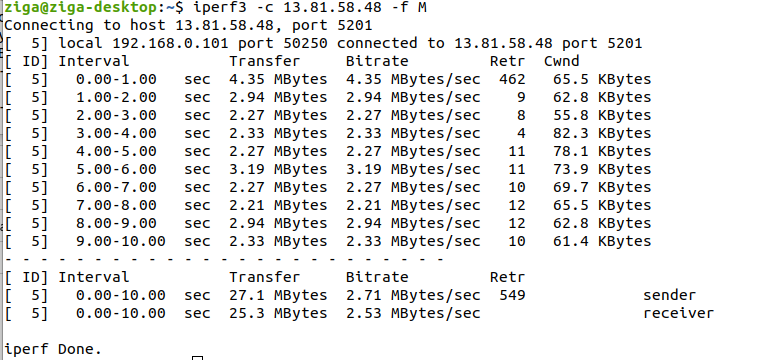
\includegraphics[scale=0.5]{Img/iperf1.png}
    \caption{test iPerf.}
    \label{fig:4_iperf1}
\end{figure}


\subsection{ioPing}
Tretji benchmark, ki sva ga izbrala je ioPing. Prednost ioPing-a naj bi bila njegova preprost, saj je zelo podoben znanemu ukazu ping, le da je namenjen testu diskovja v računalniku. Ni namenjen testiranju diskovja pod naporom, zanima ga le latenca zahtev za pisanje/branje. Le ta je izredno pomembna za podatkovne baze, ki niso pod velikim stresom zaradi števila zahtev, vendar bi njihov opazen zamik pri odzivu negativno vplival na uporabniško izkušnjo. Latenca nima velikega pomena pri večih asinhronih operacijah pisanja, saj je to veliko bolj odvisno od prepustnosti diska. Zato sva pognala testa latence pri sinhronih oz. zaporednih operacijah pisanja in latenci pri asinhronih operacijah branja. ioPing poda rezultate latence v obliki sekund, seveda pa prilagodi predpono velikosti latence. SSD, do katerega dostopa virtualka, je precej hiter in ima latenco v rangu 200 mikrosekund, kjer sta pomembni še minimum in maksimum vrednosti latence. Standardni odklon (mdev) nam pove kakšen razpon latenc lahko pričakujemo pri večini operacij. Na sliki \ref{fig:5_ioping1} so predstavljeni rezultati testa ioPing, kjer lahko vidimo odzivne čase.
\begin{figure}[H]
    \centering
    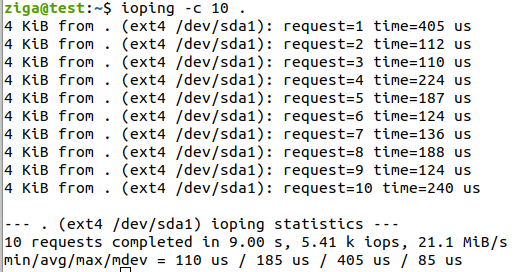
\includegraphics[scale=0.5]{Img/ioping1.png}
    \caption{test ioPing.}
    \label{fig:5_ioping1}
\end{figure}

\subsection{Fio}
Četrti benchmark, ki sva ga pognala je program fio, kar pomeni "flexible I/O". Fio je precej fleksibilen in torej bolj kompleksen program za testiranje diskovja, omogoča več specifičnih testov. Uporabljajo ga razvijalci in administratorji, za testiranje delovanje diskovja in datotečnih sistemov. Midva sva ga uporabila za test pasovne širine pisanja/branja, samo pisanja ali samo branja na disk. V povprečju neka standardna podatkovna baza dobi 3 bralne operacije za vsako pisalno operacijo, torej je razmerje med read in write operacijami 3:1. To razmerje sva uporabila pri testu kombinacije pisanja in branja. Na sliki \ref{fig:6_fio1} so predstavljeni rezultati testa Fio za read in write.

\begin{figure}[H]
    \centering
    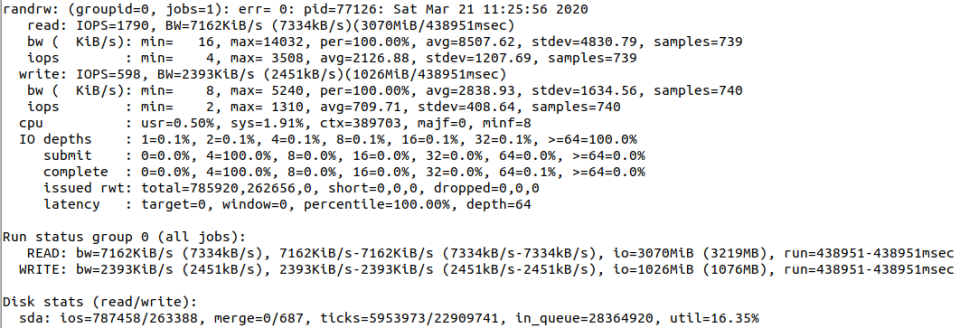
\includegraphics[scale=0.4]{Img/fio1.png}
    \caption{test Fio, R/W.}
    \label{fig:6_fio1}
\end{figure}

\subsection{Lastnosti metrik testov}

Tabela prikazuje metrike uporabljenih testov. Njihove slabosti in prednosti pred drugimi.

\begin{table}[H]
    \centering
        \begin{tabular}{ | r | r | r | r | r |} 
            \hline
            Metrike & Geekbench 3 & iPerf & ioPing & Fio  \\
            \hline
            linearnost & NE & DA & NE & NE \\
            zanesljivost & NE & DA & NE & DA  \\
            ponovljivost & DA & NE & DA & NE  \\
            enostavnost & NE & DA & DA & DA  \\
            konsistentnost & DA & DA & NE & DA  \\
            neodvisnost & NE & DA & DA & DA  \\
            \hline
        \end{tabular}
        \caption{Metrike  testov.}
    \label{table:1_chunks}
\end{table}



\section{Zmogljivost omrežnih povezav}

Merjenje zmogljivosti povezav do virtualnega računalnika sva izmerila z uporabo orodja PING in Traceroute.

\subsection{RTT}
Pri naslednjih razdelki se bo uporabljala beseda RTT, katero bom definiral tukaj. RTT (angl. Round Trip Time) ali po slovensko čas povratnega potovanja. Z besedo opišemo čas, ki je potreben za pošiljanje in prihod paketa do destinacije + čas potovanja potrditve do izvora.

\subsection{Ping}
Ping je administracijsko programsko orodje, katerega se uporablja za testiranje dosegljivosti in latence nekega omrežja preko IP protokola. Ping meri RTT sporočil poslanih od izvora do destinacije. Deluje na protokolu ICMP, kateri pošlje zahtevo in počaka na odziv.

\subsection{TraceRoute}
TraceRoute je orodje, ki se uporablja za prikaz poti od izvora do destinacije preko protokola IP. Zgodovina skokov paketa je shranjena kot RTT paketov prejetih od vsakega naslednjega vozlišča. Vsota povprečnih časov vsakega skoka je meritev celotnega časa potrebnega za vzpostavitev povezave.

\subsection{Implementacija}
Na virtualnem računalniku je bilo potrebno nastaviti pravilo, da se računalnik odziva na ICMP pakete katere prejme. Neodzivanje na ICMP pakete se lepo vidi iz slike \ref{fig:6_traceroute1}, kjer * predstavljajo vse usmerjevalnike na poti kateri se niso odzvali. Na sliki \ref{fig:6_traceroute1} se vidi testiranje iz lokacije Kranja, medtem ko na sliki \ref{fig:6_traceroute2} lahko vidimo testiranje iz lokacije Brezovica pri Ljubljani. Virtualni računalnik se nahaja na Nizozemskem zato je zadnjih nekaj skokov skoraj enakih, razlikujejo se le v številkah serverja, skozi katerega so paketi potovali. Na lokaciji Brezovica pri Ljubljani je prihodna/odhodna hitrost 100/10, na 
lokaciji Kranj pa 50/5. 

\begin{figure}[H]
    \centering
    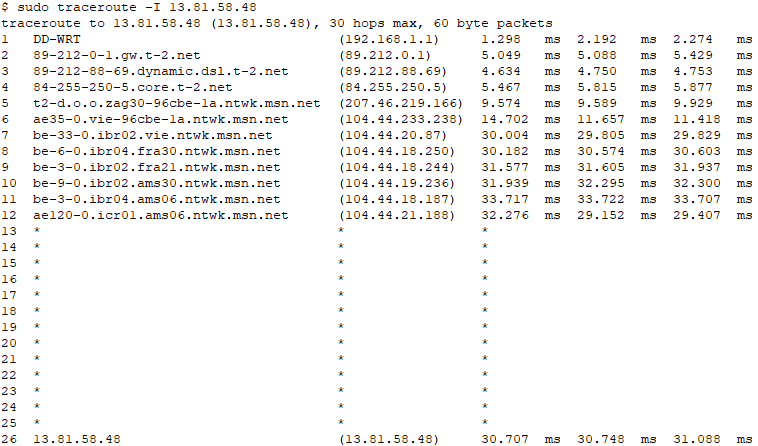
\includegraphics[scale=0.45]{Img/traceroute1.png}
    \caption{Prikaz poti iz Kranja do virtualnega računalnika.}
    \label{fig:6_traceroute1}
\end{figure}

\begin{figure}[H]
    \centering
    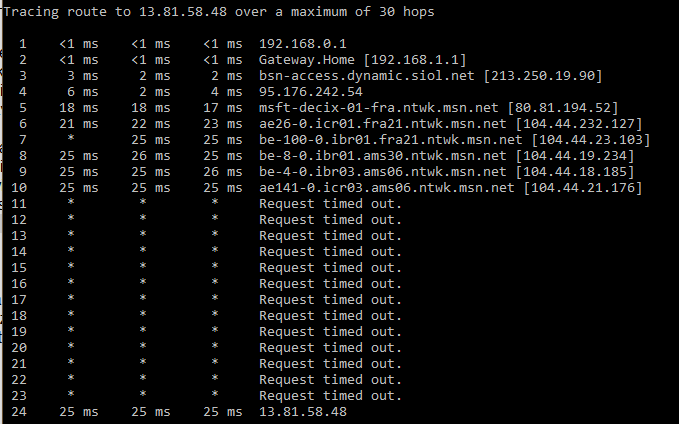
\includegraphics[scale=0.5]{Img/traceroute2.png}
    \caption{Prikaz poti iz Brezovice pri Ljubljani do virtualnega računalnika.}
    \label{fig:6_traceroute2}
\end{figure}


\subsection{Umetno breme}

Za bolj podrobno testiranje omrežja sva pripravila 2 programa. Prvi program iz lokalnega računalnika pošilja 2MB veliko datoteko, v tem programu lahko tudi določimo interval pošiljanja datoteke. Drugi program pa je treba pognati na najinem virtualnem računalniku na katerem sprejema datoteko in po uspešnem sprejemu pošlje čas prejetja, katerega prvi program izpiše.
Cilj programov je testirati hitrost procesiranja datoteke brez zapisovanja na disk.
Na sliki \ref{fig:7_breme1} lahko vidimo čase pošiljanja na 5 sekund z zelo malo nihanja. Zelo malo nihanja je zato, ker ima virtualni računalnik, ki prejema datoteke dovolj časa da stvari procesira. 

\begin{figure}[H]
    \centering
    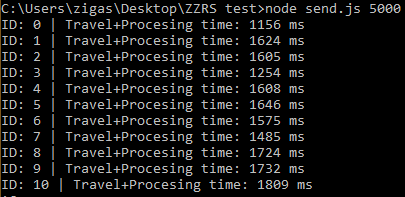
\includegraphics[scale=0.8]{Img/breme1.png}
    \caption{Časi pošiljanja na 5 sekund.}
    \label{fig:7_breme1}
\end{figure}

Če zmanjšamo interval pošiljanja na 0.5 sekunde se časi povečajo, saj virtualni računalnik nima dovolj hitrega procesiranja datotek in zaradi tega prihaja do zamud. To lahko vidimo tudi na sliki \ref{fig:7_breme2}, kjer se je čas prejemanja iz povprečno 1.2 sekunde povečal na povprečno 7 sekund.

\begin{figure}[H]
    \centering
    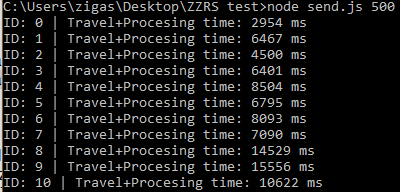
\includegraphics[scale=0.8]{Img/breme2.png}
    \caption{Časi pošiljanja na 0.5 sekunde.}
    \label{fig:7_breme2}
\end{figure}

Na zadnji sliki \ref{fig:7_breme3} lahko vidimo da je idealen čas pošiljanja datotek na približno 900 milisekund ali 0.9 sekunde. Idealen je zaradi tega, ker se datoteke pošiljajo z najhitrejšim intervalom z majhnim povprečnim časom.

\begin{figure}[H]
    \centering
    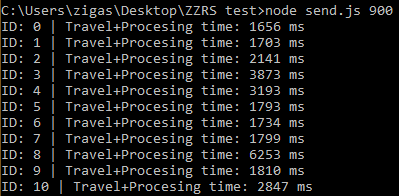
\includegraphics[scale=0.8]{Img/breme3.png}
    \caption{Časi pošiljanja na 0.9 sekunde.}
    \label{fig:7_breme3}
\end{figure}

\section{Zmogljivost diskovnega sistema}

Po sprejemu datoteke od pošiljatelja, sprejemnik pošlje svoj odgovor, datoteka pa ostane le v pomnilniku in se ne zapiše na disk. Da bi testirala tudi hitrost pisanja datotek na disk, sva ustvarila več datotek različnih velikosti, vsako od njih večkrat poslala na virtualni računalnik, ter jo po sprejetju tudi zapisala na disk. Merila sva čas od začetka zapisovanja do konca zapisovanja vsake datoteke, potrebno pa je upoštevati, da je disk, ki ga ima virtualni računalnik na voljo, precej hiter SSD.

\begin{table}[H]
	\centering
	\begin{tabular}{ | r | r | r | r | }
		\hline
		Čas pošiljanja & Min [ms] & Povprečje [ms] & Max [ms]  \\
		\hline
		1 MB & 1751 & 2273 & 2945 \\
		2 MB & 3377 & 3830 & 4589 \\
		5 MB & 3918 & 4012 & 4277 \\
		10 MB & 8208 & 8356 & 8532 \\
		20 MB & 17019 & 17160 & 17371 \\
		40 MB & 34819 & 35094 & 35439 \\
		\hline
	\end{tabular}
	\caption{Metrike  testov.}
	\label{table:1_chunks}
\end{table}

Najprej sva za vsako prejeto datoteko v pomnilniku na virtualnem računalniku ustvarila novo datoteko na disku. Povprečni časi zapisovanja so precej nizki zaradi SSD diska, odstopanja pa so razmeroma velika.

\begin{table}[H]
	\centering
	\begin{tabular}{ | r | r | r | r | }
		\hline
		Čas shranjevanja & Min [ms] & Povprečje [ms] & Max [ms]  \\
		\hline
		1 MB & 1 & 1.3 & 4 \\
		2 MB & 1 & 1.73 & 2 \\
		5 MB & 3 & 3.36 & 4 \\
		10 MB & 6 & 6.8 & 8 \\
		20 MB & 12 & 14.7 & 22 \\
		40 MB & 27 & 30.3 & 34 \\
		\hline
	\end{tabular}
	\caption{Metrike  testov.}
	\label{table:1_chunks}
\end{table}

Zanimivi so rezultati, ki sva jih dobila, ko sva vsako prejeto datoteko v pomnilniku zapisala v isto datoteko na disku. Seveda sva prepisala vsebino prejšnje prejete datoteke. Povprečni čas se je namreč močno podaljšal, minimum pa je ostal podoben prejšnjemu. Ni nama povsem jasno, zakaj se to zgodi, vendar je odstopanje od pisanja vsakič v novo datoteko preveliko, da bi ga lahko zanemarili.

\begin{table}[H]
	\centering
	\begin{tabular}{ | r | r | r | r | }
		\hline
		Čas shranjevanja & Min [ms] & Povprečje [ms] & Max [ms]  \\
		\hline
		1 MB & 1 & 1.3 & 2 \\
		2 MB & 2 & 2.3 & 5 \\
		5 MB & 4 & 24.6 & 91 \\
		10 MB & 9 & 63.3 & 112 \\
		20 MB & 18 & 192.3 & 225 \\
		40 MB & 80 & 255.9 & 348 \\
		\hline
	\end{tabular}
	\caption{Metrike  testov.}
	\label{table:1_chunks}
\end{table}

\section{Zmogljivost procesorja}

V tem razdelku bova testirala zmogljivost procesorja na virtualnem računalniku in na domačih lokacijah.


\subsection{Opis programa}

Program, ki bo testiral zmogljivost sva napisala sama. Program deluje na enem jedru procesorja. ne uporablja diskovnih pogonov.
Osnovna naloga programa je, da z matematično intenzivnim problemom testira hitrost procesorja za kar sva v najinem programu pripravila 2 taka problema. Oba problema uporabljata zelo malo dinamičnega pomnilnika in oba sta implementirana z algoritmoma, ki imata časovno zahtevnost O(n). Vsak algoritem se kliče večkrat, zaradi tega je časovna zahtevnost celotnega programa O(n\textsuperscript{2}). Ko se program zaključi se izpiše čas izvajanja enega in drugega algoritma, nato pa izpiše še skupni čas izvajanja obeh problemov.



\subsection{Algoritem za faktorizacijo}

Prvi algoritem za vsa števila na intervalu [10050000, 10050500] izračuna faktoriteto (npr. 5! = 120). Algoritem ne uporablja nobenih izblojšav s katerimi se lahko pohitri njegovo delovanje. Implementacijo algoritma lahko vidite spodaj.

\begin{lstlisting}[language=C++, caption=Algoritem faktoritet, label={lst:alg1}]
void factorialTEST()
{
    long N = 10050000;

    long iterations = 500;

	for(int i=0;i<iterations;i++)
	{
		long c, n = N, f = 1;
		for (c = 1; c <= n; c++)
			f = f * c;

		n++;
	}
}
\end{lstlisting} 

Algoritem za faktorizacijo naredi 500 ponovitev. Pri vsaki ponovitvi se naredi N+1 primerjav, C+2 seštevanj in N množenj. Začetno število N za izračun faktoritete je 10050000. Število za izračun se pri vsaki ponovitvi poveča za 1. Algoritem uporablja podatkovne strukture tipa long, kar je pri vseh računalnikih na katerih se je testiral 64-bitov. 

\subsection{Algoritem za iskanje praštevil}

Drugi algoritem za vsa števila na intervalu [10050000, 10055000] preveri če je število praštevilo. Algoritem ne uporablja nobenih izblojšav s katerimi se lahko pohitri njegovo delovanje. Implementacijo algoritma lahko vidite spodaj.

\begin{lstlisting}[language=C++, caption=Algoritem faktoritet, label={lst:alg2}]
bool isPrime(int n)
{
    if (n <= 1)
        return false;

    for (int i = 2; i < n; i++)
        if (n \% i == 0)
            return false;

    return true;
}


void primeTEST()
{
	long N = 10050000;

	long iterations = 5000;

	for(int i=N;i<N+iterations;i++)
	{
		isPrime(i);
	}
}
\end{lstlisting} 


Algoritem za preverbo praštevil naredi 5000 ponovitev. Pri vsaki ponovitvi se naredi v najslabšem primeru N primerjav, N+1 seštevanj in N deljenj. Začetno število N za preverbo pripadnosti praštevilom je 10050000. Število za izračun se pri vsaki ponovitvi poveča za 1. Algoritem uporablja podatkovne strukture tipa long in int, kar je pri vseh računalnikih na katerih se je testiral za tip long 64-bitov za tip int pa 32-bitov. 



\subsection{Rezultati meritev}

Program sva pognala tako na najinih računalnikih, na prenosnem in osebnem računalniku, kot seveda tudi na virtualnem računalniku na Azure platformi. Ročno sva za vsak slučaj preverila, da program uporablja dejansko samo eno CPU jedro, malo pomnilnika in ne piše na disk, kar sva storila z uporabo sistemskega monitorja. Rezultati meritev:

\begin{figure}[H]
	\centering
	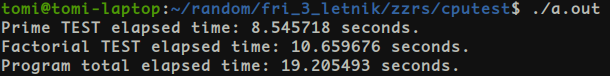
\includegraphics[scale=0.66]{Img/Tomaz_cputest.png}
	\caption{Časi izvajanja meritev na prenosnem računalniku s procesorjem Intel i5 7. generacije.}
	\label{fig:7_breme2}
\end{figure}

\begin{figure}[H]
	\centering
	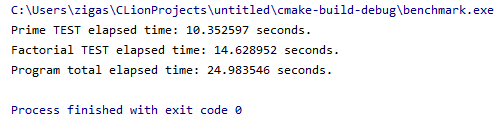
\includegraphics[scale=0.8]{Img/Ziga_cputest.png}
	\caption{Časi izvajanja meritev na osebnem računalniku s procesorjem Intel i5 3. generacije.}
	\label{fig:7_breme2}
\end{figure}

\begin{figure}[H]
	\centering
	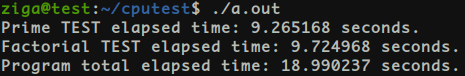
\includegraphics[scale=0.66]{Img/Azure_cputest.png}
	\caption{Časi izvajanja meritev na virtualnem računalniku na Azure platformi s procesorjem Intel Xeon Platinum 8. generacije.}
	\label{fig:7_breme2}
\end{figure}

Rezultati meritev so precej zanimivi. Čeprav je procesor v prenosnem računalniku (i5) 4 generacije novejši od procesorja v osebnem računalniku (i5), je ta sodeč po meritvah na spletu 20\% počasnejši od procesorja v osebnem računalniku. Intuicija prav tako pravi, da lahko procesor v osebnem računalniku porablja več elektrike in bi zato moral biti hitrejši, čeprav je starejše generacije. V najinih meritvah je procesor v prenosnem računalniku v vseh treh testih hitrejši od procesorja v osebnem. Razlogov za to je lahko več:

\begin{itemize}
	\item i5 ima kljub slabši splošni oceni boljšo oceno za eno jedro, kar je v teh dveh problemih relevantno
	\item i5 ima novejšo arhitekturo, ki ima določene optimizacije za ukaze, ki se uporabljajo v teh dveh problemih
	\item čeprav lahko procesor v prenosnem računalniku vleče manj elektrike, pa se testa dovolj hitro končata, da je razlika v temperaturi, ki je posledica večjega toka elektrike, minimalna in lahko tudi prenosi procesor drži polno hitrost
	\item razlika v predpomnilnikih obeh procesorjev
	\item nekaj drugega
\end{itemize}

Na to primerjavo se dobro nanaša tudi Xeon procesor na virtualnem računalniku, ki je zanimivo počasnejši v enem testu in hitrejši v drugem testu od prenosnega procesorja. Glede na to da ima Xeon boljšo oceno za eno jedro kot prenosni procesor, bi moral biti hitrejši v obeh testih. Iz primerjav najinih procesorjev in iz primerjav rezultatov na Azure platformi sklepava, da je razlika posledica arhitekturnih razlik med procesorji ali pa razlik v pomnilniku. Xeon je namreč 48 jedrni procesor in midva si ga seveda deliva z ostalimi virtualkami, ki tečejo na tem procesorju, kar lahko vpliva na delovanje predpomnilnika.

%||||||||||||||||||||||||||||| EXAMPLI ||||||||||||||||||||||||||||||||||||||||||||||||||||||||||||||||||||||||||||||||||||||||||

%Koda je predstavljena v izpisu \ref{lst:1_lst_cpu}.
%\begin{lstlisting}[caption={Primer testiranja procesorja.}, label={lst:1_lst_cpu}]
%zzrs@ZZRS:~$ sysbench --test=cpu --cpu-max-prime=20000 run
%sysbench 0.4.12:  multi-threaded system evaluation benchmark

%Running the test with following options:
%Number of threads: 1

%Doing CPU performance benchmark

%Threads started!
%Done.

%Maximum prime number checked in CPU test: 20000


%Test execution summary:
   % total time:                          29.6635s
    %total number of events:              10000
    %total time taken by event execution: 29.6616
    %per-request statistics:
       %  min:                                  2.55ms
         %avg:                                  2.97ms
        % max:                                 56.83ms
       %  approx.  95 percentile:               3.33ms

%Threads fairness:
   % events (avg/stddev):           10000.0000/0.00
    %execution time (avg/stddev):   29.6616/0.00
%\end{lstlisting}



\section{Zaključek}
Tule bo zaključek.

\section{Viri}

\begin{itemize}
	\item \href{https://www.spec.org/cloud_iaas2018/results/res2019q4/cloudiaas2018-20191113-00005.html}{SPEC Cloud R IaaS 2018}
	\item \href{https://cloudspectator.com/wp-content/uploads/2019/10/2018_Top10_NA_v1.3.pdf}{Cloud Spectator}
	\item \href{https://blog.thousandeyes.com/top-takeaways-cloud-performance-benchmark/}{Cloud Performance Benchmark}
	\item \href{https://tbri.com/tbr-difference/}{Technology Business Research, Inc.}
	\item + dodaj tiste, za katere nisi prepričan ?
\end{itemize}